\documentclass{article}
\usepackage[utf8]{inputenc}
\usepackage{graphicx}
\usepackage{titling}
% \usepackage{mathptmx} % Times New Roman font
% Da decidere meglio il font questo non mi convince
\usepackage[a4paper, top=2.5cm, bottom=2.5cm, left=2cm, right=2cm]{geometry}



\pretitle{\begin{center}
\includegraphics[width=7cm]{logo.png}\\[1em]\LARGE\bfseries}
\title{\Huge\bfseries RASD}
\author{\Large Argentini E. Battaglia S. Pantarotto A. Rosiglioni D.}




\begin{document}
\maketitle
\clearpage
\tableofcontents
\clearpage

\section{Introduction}
\subsection{Purpose}
The purpose of StudentHub is to provide a platform by students for students. Its objective is to streamline the management of student life. The platform will allow students to manage their tasks and organise their study sessions. The platform will also provide a space for students to connect with each other, share resources and collaborate on projects. The platform will also offer students a network forum where they can make announcements to find used books and private lessons, as well as share information about school events.
\subsubsection{Goals}
\begin{table}[h!]
\centering
\begin{tabular}{|c|p{10cm}|}
    \hline
    \textbf{ID} & \textbf{Description} \\
    \hline
    G1 & Allow users to create, delete, log in to and log out from an account \\
    G2 & Enable users to create, edit, move, and delete deadlines on a shared calendar \\
    G3 & Provide functionality for users to create, edit, and delete private deadlines visible only to themselves \\
    G4 & Allow users to upload, share, edit, and delete study notes on various subjects \\
    G5 & Enable users to create, manage, and delete study groups with other platform users \\
    G6 & Provide a messaging system for communication within study groups \\
    G7 & Allow users to send and receive study group invitations \\
    G8 & Provide a forum where users can create, edit, and delete announcements \\
    G9 & Enable users to comment on and interact with forum announcements \\
    G10 & Allow users to search for specific topics, notes, or announcements within the platform \\
    G11 & Provide a marketplace functionality for exchanging used academic books \\
    G12 & Enable users to offer and search for private tutoring lessons \\
    G13 & Allow users to create and share information about upcoming school events \\
    G14 & Provide notification functionality for deadline reminders and forum activity \\
    G15 & Enable users to customize their profile and privacy settings \\
    \hline
    \end{tabular}
\caption{Goals}
\label{tab:goals}
\end{table}
\clearpage
\subsection{Scope}
\subsubsection{World Phenomena}
\begin{table}[h!]
\centering
\begin{tabular}{|c|p{10cm}|}
\hline
\textbf{ID} & \textbf{Description} \\
\hline
WP1 & A student wants to create an account \\
WP2 & A student wants to delete an account \\
WP3 & A student wants to create a deadline on the shared/private calendar \\
WP4 & A student wants to move a deadline on the shared/private calendar \\
WP5 & A student wants to edit a deadline on the shared/private calendar \\
WP6 & A student wants to delete a deadline on the shared/private calendar \\
WP7 & A student wants to upload his/her study notes on a given subject \\
WP8 & A student wants to share his/her study notes on a given subject \\
WP9 & A student wants to edit his/her study notes on a given subject \\
WP10 & A student wants to delete his/her shared notes \\
WP11 & A student wants to create a studying group \\
WP12 & A student wants to invite people to his/her studying group \\
WP13 & A student wants to chat with his/her studying group \\
WP14 & A student wants to delete his/her studying group \\
WP15 & A student wants to publish an announcement on the forum \\
WP16 & A student wants to edit an announcement on the forum \\
WP17 & A student wants to delete an announcement on the forum \\
WP18 & A student wants to comment an announcement on the forum \\
WP19 & A student wants to delete a comment on the forum \\
WP20 & A student wants to share an announcement found on the forum \\
WP21 & A student wants to find documents relative to a topic \\
WP22 & A student wants to buy an academic book \\
WP23 & A student wants to offer private tutoring lessons \\
WP24 & A student wants to purchase a private tutoring lessons \\
WP25 & A student wants to customize his profile \\
\hline
\end{tabular}
\caption{World Phenomena}
\label{tab:world_phenomena}
\end{table}

\clearpage
\subsubsection{Shared Phenomena}
\begin{table}[h!]
    \centering
    \begin{tabular}{|c|p{10cm}|}
    \hline
    \textbf{ID} & \textbf{Description} \\
    \hline
    SP1 & The student creates an account on the system \\
    SP2 & The student deletes the account on the system \\
    SP3 & The student uploads a deadline in the system \\
    SP4 & The student moves a deadline in the system \\
    SP5 & The student edits a deadline in the system \\
    SP6 & The student deletes a deadline in the system \\
    SP7 & The student uploads the study notes in the system \\
    SP8 & The student uses the share function of notes provided by the system \\
    SP9 & The student edits the study notes in the system \\
    SP10 & The student deletes the study notes from the system \\
    SP11 & The student creates a study group in the system \\
    SP12 & The student invites people to the study group using the system \\
    SP13 & The student chats with the study group through the system \\
    SP14 & The student deletes the study group from the system \\
    SP15 & The student publishes an announcement on the system forum \\
    SP16 & The student edits an announcement on the system forum \\
    SP17 & The student deletes an announcement from the system forum \\
    SP18 & The student comments on an announcement in the system forum \\
    SP19 & The student deletes a comment from the system forum \\
    SP20 & The student shares an announcement using the system \\
    SP21 & The student searches a topic in the system forum \\
    SP22 & The student purchases an academic book through the system \\
    SP23 & The student offers private tutoring lessons in the system \\
    SP24 & The student books a private tutoring lesson using the system \\
    SP25 & The student customizes the profile in the system \\
    \hline
    \end{tabular}
    \caption{Shared Phenomena}
    \label{tab:shared_phenomena}
\end{table}

\subsection{Revision History}
\begin{itemize}
    \item Version 1.0 - May 4, 2025 - Initial release of the document.
\end{itemize}


\subsection{Document Structure}
% 
% ------------------------------------------------------------
% TODO: DA RISCRIVERE ALLA FINE IN BASE A COSA SI è FATTO ALLA FINE
% ------------------------------------------------------------
% 

This document is structured into 6 sections, each containing subsections that provide detailed information about the system. The sections are as follows:
\begin{itemize}
    \item \textbf{Introduction}: This section provides an overview of the system, its purpose, and goals.
    \item \textbf{Overall Description}: This section describes the system's context, stakeholders, and shared phenomena.    
    \item \textbf{Specific Requirements}: This section outlines the specific requirements for the system.
    \item \textbf{Hours Worked}: This section provides a summary of the hours worked on the project.
    \item \textbf{References}: This section lists any references used in the document.
\end{itemize}  



\clearpage
\section{Overall Description}
\subsection{Product Perspective}
\subsubsection{Scenarios}

\textbf{Scenario 1: An user creates an account and manages his own deadlines}\\
Elir, a first-year Computer Science student, creates an account on StudentHub using his university email. After verification, he adds three academic deadlines to the Calendar: a Programming assignment, a Mathematics exam, and a group project meeting. He marks the group project as "shareable" for future teammates. Elir also adds a private reminder to call home on the weekend. Later, when his Programming assignment deadline is extended, Elir easily updates it in the system.
\\ \\
\textbf{Scenario 2: An user creates an announcement on the forum}\\
Davide T., an Economics student, searches StudentHub's Forum for a specific Econometrics textbook. Not finding it, he creates an announcement requesting "Advanced Econometrics by Rosiglioni D. - 7th Edition" with his budget. Two days later, Salvo comments on his post offering to sell his copy. They arrange the exchange through direct messaging and meet at the university library. Trevisan then marks his announcement as "Resolved" with a thank-you note.
\\ \\
\textbf{Scenario 3: An user creates a study group and shares notes}\\
Pantarotto A., a Biology student, uploads his Cell Structure notes to StudentHub's "Study Resources" section with relevant tags. He then creates a "Biology Midterm Prep" study group, making it discoverable to other Biology students. Alessio invites five classmates, three of whom accept immediately. Through the group chat, he shares his notes and the team plans their study sessions for the upcoming midterm.

\clearpage
\subsubsection{Domain Model}
\begin{figure}[h]
    \centering
    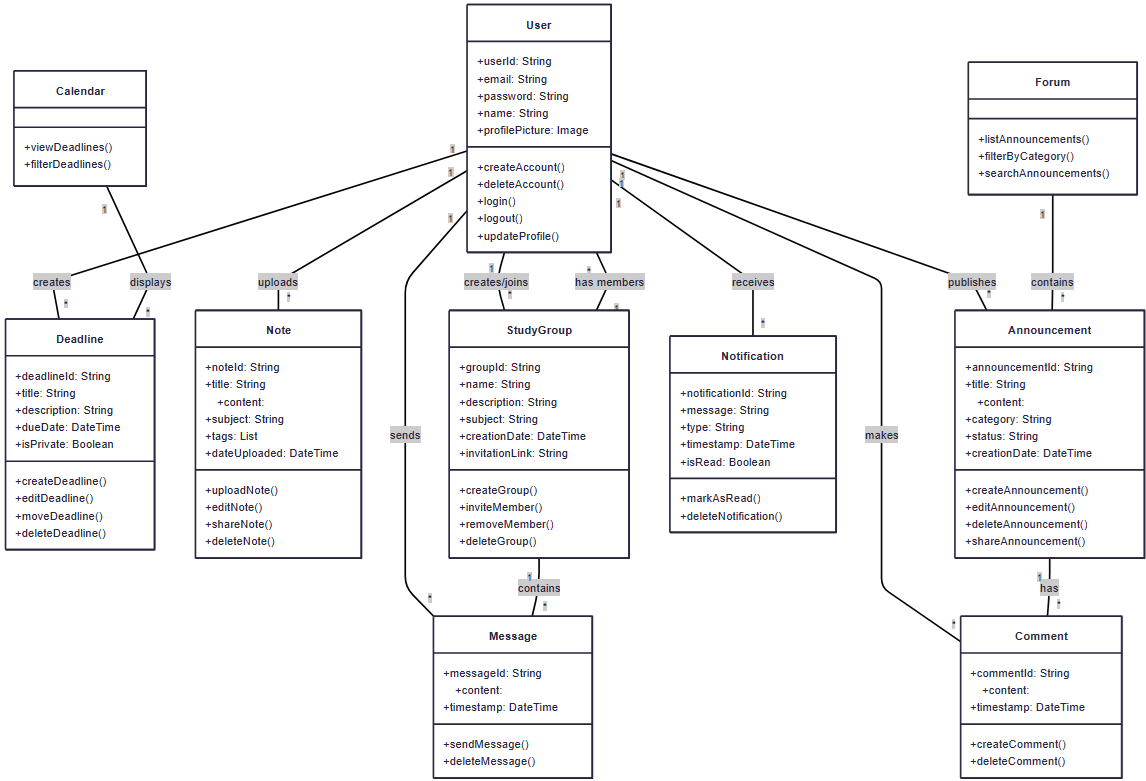
\includegraphics[width=1\textwidth]{domain_model.png}
    \caption{High level class diagram of the system}
    \label{fig:etichetta}
\end{figure}

\textbf{Domain Model Description:}\\
This domain model represents the core structure of StudentHub, a platform designed to streamline student life management. The User entity is at the core of the system, with connections to all the major components. The Calendar interface allows users to create and manage deadlines, offering options for both private and shared academic tasks. The Note entity facilitates the uploading and sharing of study materials, organised by subject and tags.
\\
StudyGroups facilitate collaboration between users, enabling members to exchange messages and coordinate study sessions. The creation of a group involves the sending of invitations to potential members. The Forum contains an Announcements section where users can post requests for books, offer tutoring services, or share event information. Should users wish to interact with announcements, they are able to do so through the 'Comments' function.
\\
The model also includes a notification system that keeps users informed about deadlines, group invitations and forum activity. The relationships between entities reflect the platform's collaborative nature, demonstrating how users interact with content and each other.
\\
This structure supports all of the identified goals of the RASD, including account management, deadline tracking, resource sharing, group collaboration, forum interactions, and marketplace functionality, creating a comprehensive ecosystem for student academic life management.





% INSERT HERE ALL OTHER POINT 2 SUBSECTIONS













\clearpage
\section{Specific Requirements}







\clearpage
\section{Effort spent}


\subsection{Argentini Elir}
\begin{center}
    \begin{tabular}{|l|r|}
    \hline
    \textbf{Task} & \textbf{Effort spent (hours)} \\
    \hline
    Introduction & 3 \\
    Overall Description & 1:30 \\
    Specific Requirements & 2 \\
    Reasoning & 3 \\
    Writing and Fixing & 3 \\
    Graphic Adjustments & 0 \\
    \hline
    \textbf{Total} & \textbf{12:30} \\
    \hline
    \end{tabular}
\end{center}

\subsection{Battaglia Salvatore}
\begin{center}
    \begin{tabular}{|l|r|}
\hline
\textbf{Task} & \textbf{Effort spent (hours)} \\
\hline
Introduction &  2 \\
Overall Description &  1:30\\
Specific Requirements &  2\\
Reasoning &  3\\
Writing and Fixing &  1\\
Graphic Adjustments &  2\\
\hline
\textbf{Total} & \textbf{11:30} \\
\hline
\end{tabular}
\end{center}

\subsection{Pantarotto Alessio}
\begin{center}
    \begin{tabular}{|l|r|}
\hline
\textbf{Task} & \textbf{Effort spent (hours)} \\
\hline
Introduction &  0\\
Overall Description &  0\\
Specific Requirements &  2\\
Reasoning &  3 \\
Writing and Fixing &  3\\
Graphic Adjustments &  1\\
\hline
\textbf{Total} & \textbf{9} \\
\hline
\end{tabular}
\end{center}

\subsection{Rosiglioni Diego}
\begin{center}
    \begin{tabular}{|l|r|}
\hline
\textbf{Task} & \textbf{Effort spent (hours)} \\
\hline
Introduction &  0\\
Overall Description &  0\\
Specific Requirements &  1\\
Reasoning &  2\\
Writing and Fixing &  1\\
Graphic Adjustments &  4\\
\hline
\textbf{Total} & \textbf{8} \\
\hline
\end{tabular}
\end{center}







\end{document}